\documentclass[aspectratio=169]{beamer}
% Shared preamble for ml/ slide decks.
% Each lecture .tex starts with:
%   \documentclass[aspectratio=169]{beamer}
%   \input{../preamble}
% Compile from inside the chapter folder so \input{../preamble} resolves.

\usetheme{default}
\usecolortheme{dove}

\setbeamertemplate{navigation symbols}{}
\setbeamertemplate{footline}{%
  \hfill{\large\insertframenumber\,/\,\inserttotalframenumber}\hspace{0.8em}\vspace{0.5em}%
}

% Project palette (existing, kept for backwards compatibility with deferred/*)
\definecolor{popblue}{RGB}{52, 101, 164}
\definecolor{sampred}{RGB}{204, 0, 0}
\definecolor{paramgreen}{RGB}{0, 140, 70}
\definecolor{warnred}{RGB}{180, 40, 40}
\definecolor{orange1}{RGB}{220, 120, 0}
\definecolor{violet1}{RGB}{120, 50, 160}
\definecolor{lightbg}{RGB}{245, 245, 250}

% Armenian flag palette (use these for any 3-color highlight; per CLAUDE.md).
% "Nice versions": slightly de-saturated from the official spec for slide use,
% so they don't burn out under projector colors. Originals kept as *_pure.
\definecolor{armred}{RGB}{200, 30, 40}      % nice red (official #D90012 muted)
\definecolor{armblue}{RGB}{30, 70, 160}     % nice blue (official #0033A0 muted)
\definecolor{armorange}{RGB}{230, 160, 30}  % nice orange (official #F2A800 muted)
\definecolor{armred_pure}{HTML}{D90012}     % official Armenian flag red
\definecolor{armblue_pure}{HTML}{0033A0}    % official Armenian flag blue
\definecolor{armorange_pure}{HTML}{F2A800}  % official Armenian flag orange

\setbeamercolor{frametitle}{fg=popblue}
\setbeamercolor{title}{fg=popblue}

\usepackage{pgfplots}
\usepackage{tikz}
\usetikzlibrary{shapes, arrows.meta, positioning, calc, decorations.pathreplacing, patterns, matrix}
\pgfplotsset{compat=1.18}
\usepackage{amsmath, amssymb, amsfonts}
\usepackage{bm}
\usepackage{dsfont}
\usepackage{array}
\usepackage{pifont}
\usepackage{colortbl}
\usepackage{fontenc}

% Callout boxes. Purely additive - existing decks are unaffected.
% Usage: \begin{tcolorbox}[colback=armblue!8, colframe=armblue, boxrule=0.6pt, arc=2pt,
%                          title=\textbf{Key idea}] ... \end{tcolorbox}
% Palette convention (ml/SLIDE_STYLE.md): armblue=key idea, armred=trap/warning,
% paramgreen=takeaway or "Next", armorange=watch-out.
\usepackage[most]{tcolorbox}

% Cleaner table rules (\toprule, \midrule, \bottomrule). Also purely additive.
\usepackage{booktabs}

% \cancel{...} for struck-through terms in derivations (added 2026-08-11 for the
% importance-sampling frame in ch11_rl, where the dynamics cancel). Purely additive.
\usepackage{cancel}

% Minimal ML notation macros (subset of slds-lmu latex-math/basic-ml.tex).
% Kept here so we don't have to inline-expand every \thetav, \xv, etc.
% when porting upstream slides.
\newcommand{\R}{\mathds{R}}
\newcommand{\N}{\mathds{N}}
\newcommand{\E}{\mathds{E}}
\newcommand{\Xspace}{\mathcal{X}}
\newcommand{\Yspace}{\mathcal{Y}}
\newcommand{\Hspace}{\mathcal{H}}
\newcommand{\D}{\mathcal{D}}
\newcommand{\Dtrain}{\mathcal{D}_{\text{train}}}
\newcommand{\Dtest}{\mathcal{D}_{\text{test}}}
\newcommand{\xv}{\mathbf{x}}
\newcommand{\yv}{\mathbf{y}}
\newcommand{\Xmat}{\mathbf{X}}
\newcommand{\id}{\mathbf{I}}
\newcommand{\thetav}{\bm{\theta}}
\newcommand{\thetah}{\hat{\bm{\theta}}}
\newcommand{\lamv}{\bm{\lambda}}
\newcommand{\fx}{f(\xv)}
\newcommand{\fxt}{f(\xv \,|\, \bm{\theta})}
\newcommand{\fxi}{f\!\left(\xv^{(i)}\right)}
\newcommand{\fh}{\hat{f}}
\newcommand{\fxh}{\hat{f}(\xv)}
\newcommand{\yh}{\hat{y}}
\newcommand{\yih}{\hat{y}^{(i)}}
% \xi clashes with the Greek letter \xi; write \xv^{(i)} inline instead.
\newcommand{\yi}[1][i]{y^{(#1)}}
\newcommand{\xyi}[1][i]{\left(\xv^{(#1)},\, y^{(#1)}\right)}
\newcommand{\thx}{\bm{\theta}^\top \xv}
\newcommand{\sumin}{\sum_{i=1}^{n}}
\newcommand{\sumjp}{\sum_{j=1}^{p}}
\newcommand{\Lxy}{L\!\left(y, \fx\right)}
\newcommand{\Lxyi}{L\!\left(\yi, \fxi\right)}
\newcommand{\risk}{\mathcal{R}}
\newcommand{\riske}{\mathcal{R}_{\text{emp}}}
\newcommand{\risket}{\mathcal{R}_{\text{emp}}(\bm{\theta})}
\newcommand{\riskt}{\mathcal{R}(\bm{\theta})}
\newcommand{\riskr}{\mathcal{R}_{\text{reg}}}
\newcommand{\argmin}{\mathop{\mathrm{arg\,min}}}
\newcommand{\argmax}{\mathop{\mathrm{arg\,max}}}
\newcommand{\eps}{\varepsilon}


\graphicspath{{fig/}{../00_shared/fig/}}

% callout boxes, matching the chapter's fcolorbox house pattern (LLM-1 to LLM-12)
\newcommand{\keybox}[1]{\fcolorbox{armblue}{armblue!8}{\parbox{0.97\linewidth}{\small #1}}}
\newcommand{\trapbox}[1]{\fcolorbox{armred}{armred!8}{\parbox{0.97\linewidth}{\small #1}}}
\newcommand{\takebox}[1]{\fcolorbox{paramgreen}{paramgreen!8}{\parbox{0.97\linewidth}{\small #1}}}
\newcommand{\watchbox}[1]{\fcolorbox{armorange}{armorange!12}{\parbox{0.97\linewidth}{\small #1}}}

\newcommand{\sectiontransition}[2]{%
  \begin{frame}[plain]
    \vfill
    \begin{center}
      {\Huge\bfseries\color{popblue} #1}\\[1.1em]
      {\large #2}
    \end{center}
    \vfill
  \end{frame}}

\newcommand{\src}[1]{{\scriptsize\color{gray} #1}}

\title{Fine-tuning on a Budget}
\subtitle{LoRA and QLoRA}
\author{}
\date{}

\begin{document}

\begin{frame}[plain]
  \titlepage
  \begin{center}\scriptsize\color{gray}
    LLM chapter, session 13. Toy numbers unless a slide says otherwise.
  \end{center}
\end{frame}

% ============================================================ WHERE WE ARE (py_src/llm_roadmap.py)
\begin{frame}{Where we are: one forward pass}
  \begin{center}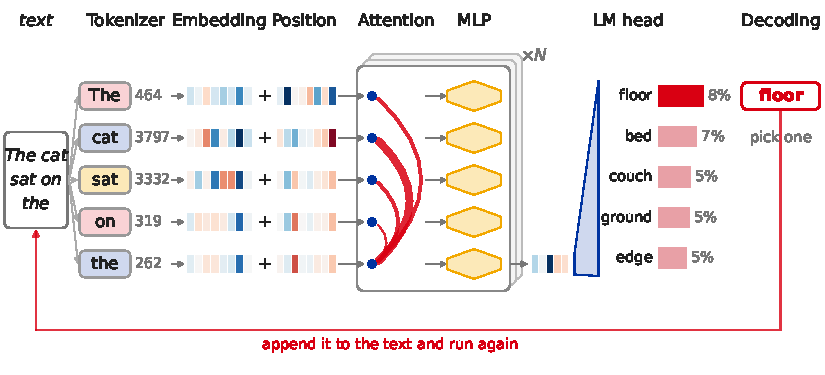
\includegraphics[width=\linewidth]{roadmap_lora_pass.pdf}\end{center}
  \vskip -2pt
  {\small The same pass. Today we change a few of its weights - cheaply.}
\end{frame}

\begin{frame}{Where we are: the life of a model}
  \begin{center}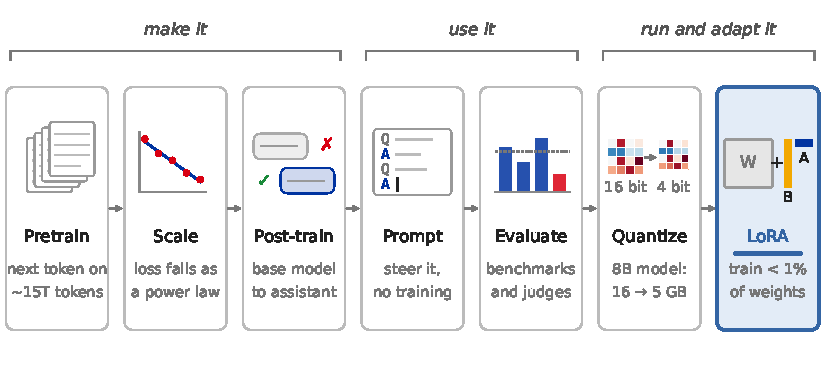
\includegraphics[width=\linewidth]{roadmap_lora_life.pdf}\end{center}
  \vskip -2pt
  {\small Today: the last box. Adapting a model to your task on hardware you can get.}
\end{frame}

% ============================================================ COLD OPEN (py_src/lora_figs.py --gpt2)
\begin{frame}{How much do you need to change?}
  \vskip 8pt
  Full fine-tuning updates every weight. For a 7B model that needs about 112 GB of memory
  (LLM-8's 16 bytes per parameter) - several big GPUs.

  \vskip 10pt
  We want GPT-2 to open every answer with ``Good question!''. Out of the box, it never does.

  \vskip 12pt
  \trapbox{\textbf{Predict first:} what share of GPT-2's 124M weights must we train to teach it
  that habit - 50\%? 10\%? 1\%?}
\end{frame}

\begin{frame}{0.24\% was enough}
  \vskip 4pt
  \begin{columns}[c]
    \column{0.52\textwidth}
      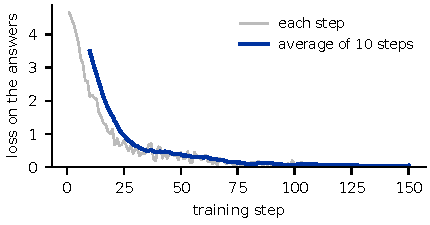
\includegraphics[width=\linewidth]{lora_loss.pdf}
    \column{0.46\textwidth}
      {\small Real run on this laptop, cached GPT-2, written by hand (no library): 294,912 new
      weights (0.24\%) trained for 150 steps on 32 short conversations; everything else frozen.
      A few minutes of CPU.

      \vskip 6pt
      20 questions it never saw, answers opening with ``Good question!'':
      \textbf{0 of 20} before, \textbf{20 of 20} after. (Closest guess: 1\%; the count is derived
      in a few pages.)}
  \end{columns}

  \vskip 6pt
  {\small ``What is the capital of Italy?'' $\to$ ``Good question! Rome.'' \quad But ``How many wheels
  does a bicycle have?'' $\to$ ``Good question! Eight.'' - wrong: the habit transferred, the facts
  did not improve.}

  \vskip 4pt
  \keybox{That is LoRA. Today: how a quarter of a percent can be enough, and how to do it to a
  7B model on a free GPU.}
\end{frame}

\begin{frame}{Outline}
  \tableofcontents
\end{frame}

% ============================================================ 1. SHOULD YOU FINE-TUNE?
\section{Should you fine-tune?}
\sectiontransition{Should you fine-tune?}{Usually not first.}

\begin{frame}{The ladder}
  \vskip 6pt
  \begin{enumerate}
    \item \textbf{Prompt} (LLM-10): free, instant, reversible. Try it first.
    \item \textbf{Give it documents} (RAG): for facts it does not know or that change.
    \item \textbf{Fine-tune}: for a format, a style, a narrow task done thousands of times.
  \end{enumerate}

  \vskip 8pt
  {\small A fourth option for a whole new domain or language: \textbf{continued pretraining} -
  LLM-7's objective on more text, for example Armenian news (as arm-gemma did, LLM-11).}

  \vskip 8pt
  \watchbox{Fine-tuning teaches \emph{how} to answer far better than \emph{what} is true (LIMA,
  LLM-9). Our demo changed GPT-2's habit, not its knowledge: asked for the capital of Armenia, it
  now answers politely - ``Good question! Ararat.'' (It is Yerevan.)}
\end{frame}

% ============================================================ 2. LORA
\section{LoRA}
\sectiontransition{LoRA}{Train a small correction, not the whole matrix.}

\begin{frame}{The bill for full fine-tuning}
  \vskip 6pt
  \begin{itemize}
    \item Every trained weight needs its gradient and Adam's two running averages, plus a 32-bit
      copy: 16 bytes per parameter (LLM-8).
    \item A 7B model: $7 \times 10^9 \times 16 = 112$ GB, before activations.
    \item And every fine-tuned version is a full new copy of the model.
  \end{itemize}

  \vskip 10pt
  \keybox{The memory goes to the parameters you train. Train fewer, and most of the bill
  disappears.}
\end{frame}

\begin{frame}{W + BA}
  \begin{center}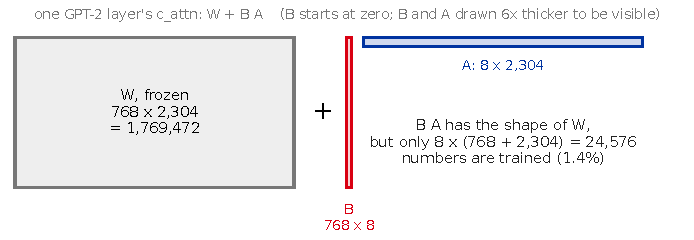
\includegraphics[width=0.84\linewidth]{lora_ba.pdf}\end{center}
  \vskip -4pt
  \begin{itemize}
    \small
    \item Keep $W$ frozen. Learn its \emph{change} as a product of two thin matrices, $\Delta W =
      B A$: a matrix of \textbf{rank} 8 at most (every row a mix of 8 directions). GPT-2's layer
      computes $x W$, so with the adapter (the pair $B$, $A$): $\; x W + \frac{\alpha}{r}\, x B A$.
    \item $A$ starts random, $B$ at zero: $BA = 0$, so step 0 is \emph{exactly} the base model (our
      run: largest logit difference 0). Not both zero - then neither would get a gradient.
    \item $\alpha / r$ scales the update; ours, $16 / 8 = 2$. Change $r$ and $\alpha$ keeps the
      update's size, so the learning rate need not be retuned.
  \end{itemize}
\end{frame}

\begin{frame}{The count, by hand}
  \vskip 6pt
  One GPT-2 layer's attention matrix \texttt{c\_attn}, $768 \times 2{,}304$:
  \vskip 4pt
  \begin{center}
  \begin{tabular}{lr}
    \toprule
    the matrix itself & $768 \times 2{,}304 = 1{,}769{,}472$ \\
    a rank-8 LoRA: $B$ and $A$ & $8 \times (768 + 2{,}304) = 24{,}576$ \quad (1.4\%) \\
    the same in all 12 layers & $12 \times 24{,}576 = 294{,}912$ \\
    share of GPT-2's 124,439,808 & \textbf{0.24\%} \\
    \bottomrule
  \end{tabular}
  \end{center}

  \vskip 8pt
  \keybox{Only these are trained, so only these need gradients and Adam's state. The 16 bytes per
  parameter now apply to 0.3M weights, not 124M.}
\end{frame}

\begin{frame}{Why a low rank is enough}
  \vskip 6pt
  \begin{itemize}
    \item A fine-tune does not rebuild the model; it nudges it. LoRA's hypothesis: that nudge,
      $\Delta W$, has a low ``intrinsic rank''.
    \item Hu et al. (2021) tested it on GPT-3: adapting the attention matrices, accuracy on their
      tasks was already good at rank 1 and barely changed above it.
    \item On GPT-3 175B, LoRA cut the trainable parameters 10,000$\times$ and GPU memory 3$\times$,
      with quality on par with full fine-tuning.
  \end{itemize}

  \vskip 10pt
  \watchbox{``On par'' was measured on tasks like the ones in the paper. A task far from what the
  base model knows may need a higher rank, more matrices - or full fine-tuning.}
\end{frame}

\begin{frame}{Which matrices, and after training}
  \vskip 6pt
  \begin{itemize}
    \item The original LoRA adapted attention only. QLoRA (2023) found it needed adapters on
      \textbf{every} linear layer, attention and MLP, to match full fine-tuning. Our demo used
      \texttt{c\_attn} only - enough for a habit.
    \item \textbf{Merge}: $W' = W + \frac{\alpha}{r} B A$ is a normal matrix again, so the merged
      model is as fast as the original. In our run, merging changed no logit by more than
      0.0002 (rounding). With a 4-bit base (QLoRA): merge into the 16-bit weights, then quantize
      again.
    \item Or keep the adapters separate: one base model, a small file per task, swapped in.
  \end{itemize}
\end{frame}

% ============================================================ 3. QLORA
\section{QLoRA}
\sectiontransition{QLoRA}{LoRA on a 4-bit base.}

\begin{frame}{Shrink the frozen part too}
  \begin{columns}[c]
    \column{0.58\textwidth}
      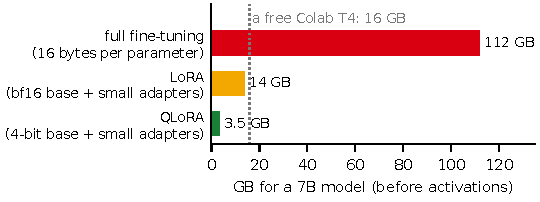
\includegraphics[width=\linewidth]{lora_memory.pdf}
    \column{0.40\textwidth}
      {\small With LoRA, the frozen base still has to sit in memory: 14 GB in 16-bit for a 7B
      model - leaving almost nothing of a 16 GB GPU for activations and the adapters' Adam state.
      QLoRA stores the base in 4 bits (LLM-12): 3.5 GB of raw weights, about 12 GB to spare.

      \vskip 4pt
      The adapters train in 16-bit; the base is turned back into 16-bit on the fly for each
      multiply.}
  \end{columns}

  \vskip 8pt
  \takebox{A 7B model can be fine-tuned on a free Colab T4 with 16 GB. Dettmers et al. (2023)
  fine-tuned a 65B model on a single 48 GB GPU, matching 16-bit fine-tuning.}
\end{frame}

\begin{frame}{What QLoRA added}
  \vskip 6pt
  \begin{itemize}
    \item \textbf{NF4}, a 4-bit format whose 16 levels sit at the quantiles of a normal
      distribution: each level covers the same share of weights, so the levels are dense where
      trained weights are dense (near 0). Blocks with a scale each, as in LLM-12.
    \item \textbf{Double quantization}: the block scales are themselves quantized - about 0.37
      bits per parameter saved, some 3 GB on a 65B model.
    \item \textbf{Paged optimizers}: when GPU memory spikes, optimizer state is paged out to CPU RAM
      and back - slower for a moment, but no crash.
  \end{itemize}

  \vskip 10pt
  \keybox{QLoRA's Guanaco models reached 99.3\% of ChatGPT's level on the Vicuna benchmark (a
  judge-based test, LLM-11) - from a single GPU.}
\end{frame}

% ============================================================ 4. THE RECIPE
\section{The recipe}
\sectiontransition{The recipe}{What goes wrong, and how to check.}

\begin{frame}{The recipe}
  \vskip 4pt
  \begin{itemize}
    \item \textbf{Data}: a few hundred to a few thousand clean examples beat many messy ones
      (LIMA, LLM-9). Ours: 32.
    \item \textbf{The chat template must match} (LLM-9): train and use the model in the same
      format, special tokens included.
    \item \textbf{Score only the answers}: the loss skips the prompt's tokens (our run did this).
    \item \textbf{Evaluate before and after} on held-out questions (LLM-11) - as the 20 unseen
      questions did here.
    \item \textbf{Watch for catastrophic forgetting}: a model fine-tuned hard on one task can get
      worse at others. Test a few general questions too.
  \end{itemize}

  \vskip 6pt
  \watchbox{Before converting a fine-tuned model for a laptop engine (LLM-12), merge the adapter
  into the weights: not every engine loads separate adapters.}
\end{frame}

% ============================================================ CLOSE
\begin{frame}{Recap}
  \small
  \begin{itemize}
    \item \textbf{Fine-tune last}: prompt, then documents, then fine-tune - for format and style,
      not facts.
    \item \textbf{LoRA}: freeze $W$, learn $\Delta W = BA$ of low rank; $B = 0$ so step 0 is the
      base model. 0.24\% of GPT-2's weights taught it a new habit.
    \item \textbf{Merge} for zero extra cost at run time, or keep small adapters per task.
      Fine-tuning can cause forgetting: test general questions too.
    \item \textbf{QLoRA}: the frozen base in 4-bit NF4 - a 7B model fits a 16 GB GPU.
    \item \textbf{The recipe}: clean data, the right template, answers-only loss, evaluate before
      and after.
  \end{itemize}
\end{frame}

\begin{frame}{Next on the map}
  \begin{center}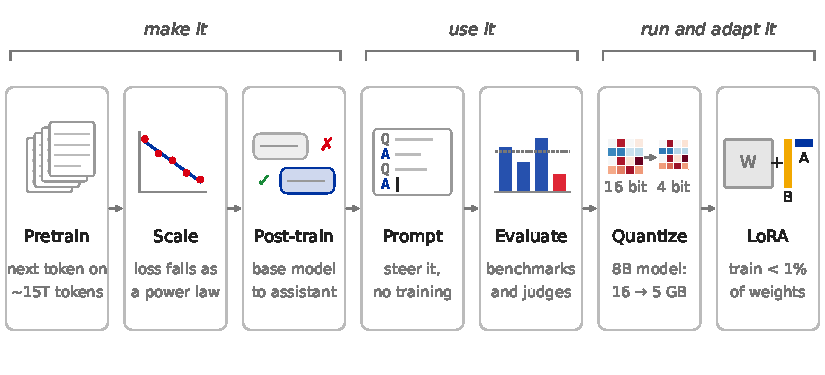
\includegraphics[width=\linewidth]{roadmap_anatomy_2026_life.pdf}\end{center}
  \vskip -2pt
  {\small Next (LLM-14): what changed inside a 2026 LLM since GPT-2, and what each change costs.}
\end{frame}

\begin{frame}{Sources \& further reading}
  \footnotesize
  \begin{itemize}
    \item Hu et al. (2021), ``LoRA: Low-Rank Adaptation of Large Language Models''.
    \item Dettmers et al. (2023), ``QLoRA: Efficient Finetuning of Quantized LLMs''.
    \item Aghajanyan et al. (2020), ``Intrinsic Dimensionality Explains the Effectiveness of Language
      Model Fine-Tuning''.
    \item Zhou et al. (2023), ``LIMA''; Gururangan et al. (2020), ``Don't Stop Pretraining''.
  \end{itemize}
  \vskip 2pt
  \src{Figures: \texttt{py\_src/lora\_figs.py}. Real: the LoRA run on the cached GPT-2 (written by
  hand, one run, seed 509). By hand: the parameter counts and the memory bars.}
\end{frame}

\end{document}

% ============================================================================
% Provenance:
%   Deck: LLM-13 LoRA and QLoRA (14_llms), session 13. Built 2026-10-06 from LLM13_lora_OUTLINE.md,
%   which follows the critique in LLM_CHAPTER_PLAN.md (LLM-13) and the queue (instructor: "do all
%   queue items"): library-free slides (D5, DECISIONS #75); the local LoRA demo on the cached GPT-2
%   (written by hand in PyTorch, no PEFT); D6 (the practical's base model) still open - measured
%   2026-10-06: only GPT-2 is fully cached (Qwen2.5-0.5B-Instruct: tokenizer only; arm-gemma-e4b:
%   nothing), so a decision needs a download - the instructor's call.
%   Sources ported: llm_training 03 (LoRA: intrinsic rank, W_q/W_v, merge) and 12 (QLoRA: NF4,
%   double quantization, paged optimizers, every linear layer); dl4nlp 07 (PEFT). Cut: the PEFT
%   family frame, DoRA and friends, the Unsloth / Ollama export steps (tool-specific; #74/#75).
%   Facts checked 2026-10-06: the LoRA and QLoRA abstracts (10,000x / 3x; 65B on one 48 GB GPU,
%   99.3% of ChatGPT on Vicuna; NF4, double quantization, paged optimizers).
%   Every printed number is asserted in py_src/lora_figs.py.
%   The run (2026-10-06): step-0 gap 0.0; 0 -> 20 of 20; merge gap 1.24e-4; the bicycle -> "Eight" and
%   Armenia -> "Ararat" outputs shown as they came. One 17-minute machine stall between steps 110
%   and 120 (the log's 1,265 s); the steps themselves took about 4 minutes, so the slide says "a few".
%   STUDENT REVIEW 2026-10-06 (one Sonnet agent, rendered PNGs only; ~77k tokens, 66 s). Caught a real
%   error: the layer was written W x + B A x, but GPT-2's c_attn computes x W (W is 768 x 2,304) - now
%   x W + (alpha/r) x B A. Applied: A random and B zero, and why not both; alpha/r = 16/8 = 2; rank and
%   adapter defined; the wrong demo answers marked as wrong; "on their tasks" for Hu et al.;
%   merging into a 4-bit base; why 14 GB does not fit a 16 GB T4; NF4's equal-share levels; double
%   quantization's 0.37 bits (local QLoRA deck); paged optimizers to CPU RAM; catastrophic
%   forgetting; a legend on the loss plot.
% ============================================================================
